
\section{Results}

\nancomment{
	figures are stored in google drive, the link is pinned in slacker;
	%https://drive.google.com/open?id=0B4jePsYXW6SSTTRLb0FHVXVjNUk
	figures/*.pdf}\\

\subsection{Image}

\subsubsection{Growth  of images at docker registry}

%1. Fig: The total number of images increases from May 30th to Sept. XXX (May 30th - July 11th)(July 11th - Sept. 1)
%!!!!!replace image with repositories.
Figure~\ref{fig_image_growth} show the total number of images in Docker hub increases from May 30th to Sept. 17th 2017. As discussed in~\cite{XXX}, Crawler searched for `/' by using Docker hub search engine, crawled the web page, and obtained the totoal number of non-official public repositories in Docker hub each day. By summing both official image count and non-official image count, we got the total number of images in Docker hub each day. Figure~\ref{fig_image_growth_first} shows the total number of images in Docker hub each day from May 30th to July 11th. The total number of images increased from xxx to xxx, with almost 1,300 images created per day.

\begin{figure}
  \centering
  % Requires \usepackage{graphicx}
  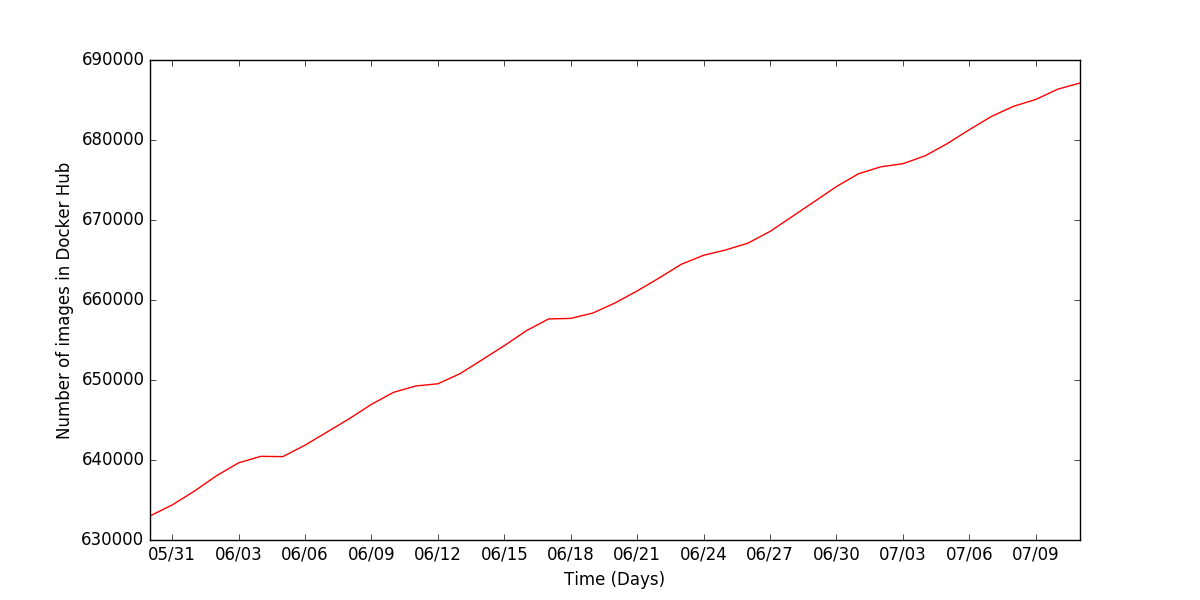
\includegraphics[width=0.5\textwidth]{graphs/image_growth}\\
  \caption{Total number of images in Docker hub from May 30th to Sept. XXX}\label{fig_image_growth}
\end{figure}

A interesting observation is that Crawler can get a similar list of images if we replace `/' with `*'. Note that from 5/30/2017-7/11/2017, Crawler used above method to obtain the total amount of images in Docker Hub. But after 7/11/2017, the Docker Hub removed the index of `/'. Thus, currently we search for `*' instead of `/' to obtain a list of non-official public images. As shown in figure~\ref{fig_image_growth_second}, the total number of images increased from xxx to xxx, with almost xxxx images created per day.

\subsubsection{Image popularity distribution}

\nancomment{TODO: 1. Fig: The avg. number of images pulled per day from May 30th to Sept. 1}

%2. Fig: The total number of images pulled by May 30th.
Figure~\ref{fig_pull_cnt_total} shows the image popularity distribution. The x-axies show the total number of pull count for each image ranges from 0 to 250. The blue line shows the cumulative distribution of total number of pull count per image while the red line shows the frequency distribution of total number of pull count per image. 85\% of the images are pulled than 250 totally. The greatest pull count is xxx which is official image~\textit{nginx}. About 12,000 has a pull count of ~xxx.

\begin{figure}
	\centering
	% Requires \usepackage{graphicx}
	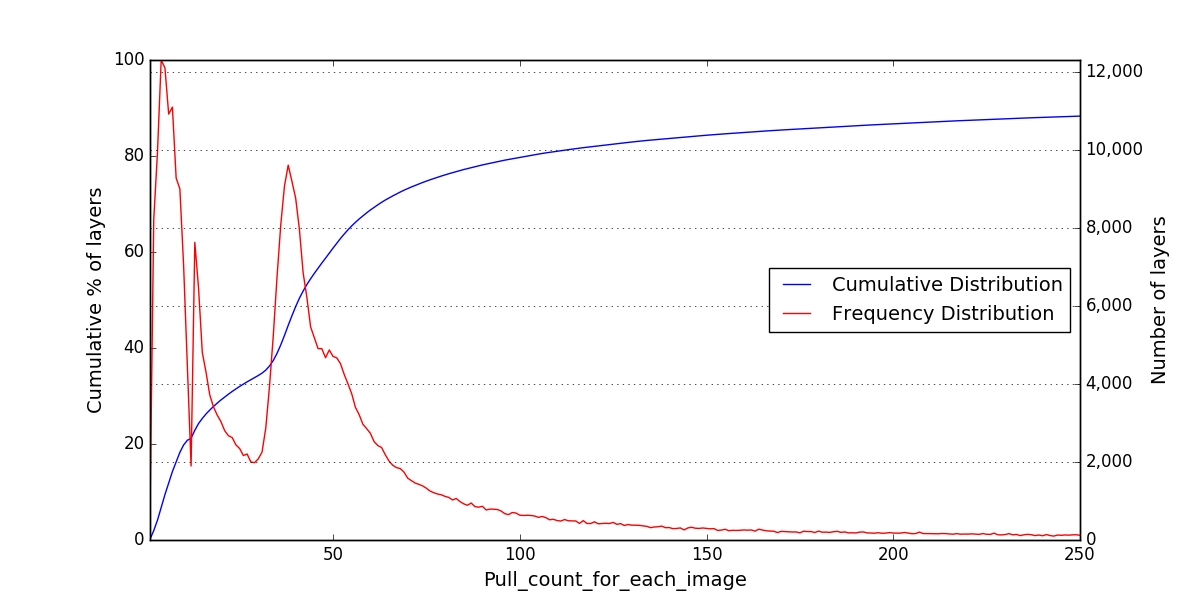
\includegraphics[width=0.5\textwidth]{graphs/2distributionPull_count_for_each_image.png}\\
	\caption{Total number of pull count for each image by May 30th}\label{fig_pull_cnt_total}
\end{figure}


\subsubsection{Image size distribution}

%1. Fig: Image compression size as the sum of its gzip compressed layer size.
%56\%
Figure~\ref{fig_image_size_compression} shows the image compression size distribution. The x-axies shows the image compression size which is the sum of its compressed layer size. The blue line shows the cumulative distribution of image compression size. 56\% of images are less than 50 MB. xxx of images are less than xxx MB. The biggest image is xxx GB while around 120,000 of images are less than ~2 MB. We can conclude that most of the images in Docker hub are small images, less than xxx MB.

\begin{figure}
	\centering
	% Requires \usepackage{graphicx}
	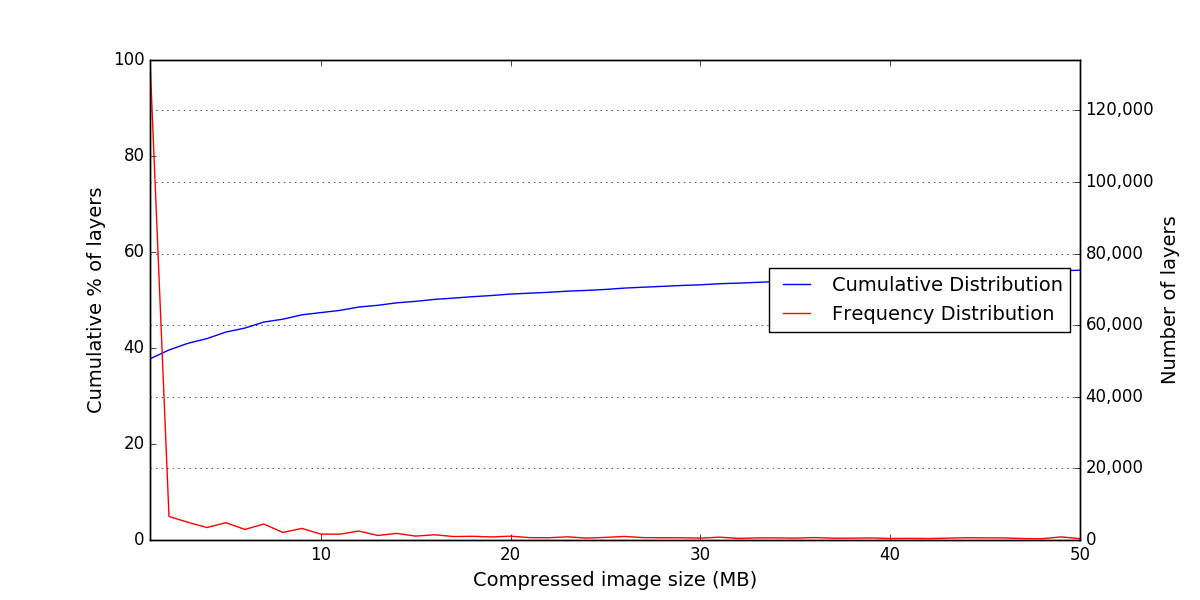
\includegraphics[width=0.5\textwidth]{graphs/distributionCompressed_image_size_(MB)}\\
	\caption{Image compression size distribution}\label{fig_image_size_compression}
\end{figure}

2. Fig: Image Decompressed size as the sum of its layer decompression size.

\begin{figure}
	\centering
	% Requires \usepackage{graphicx}
	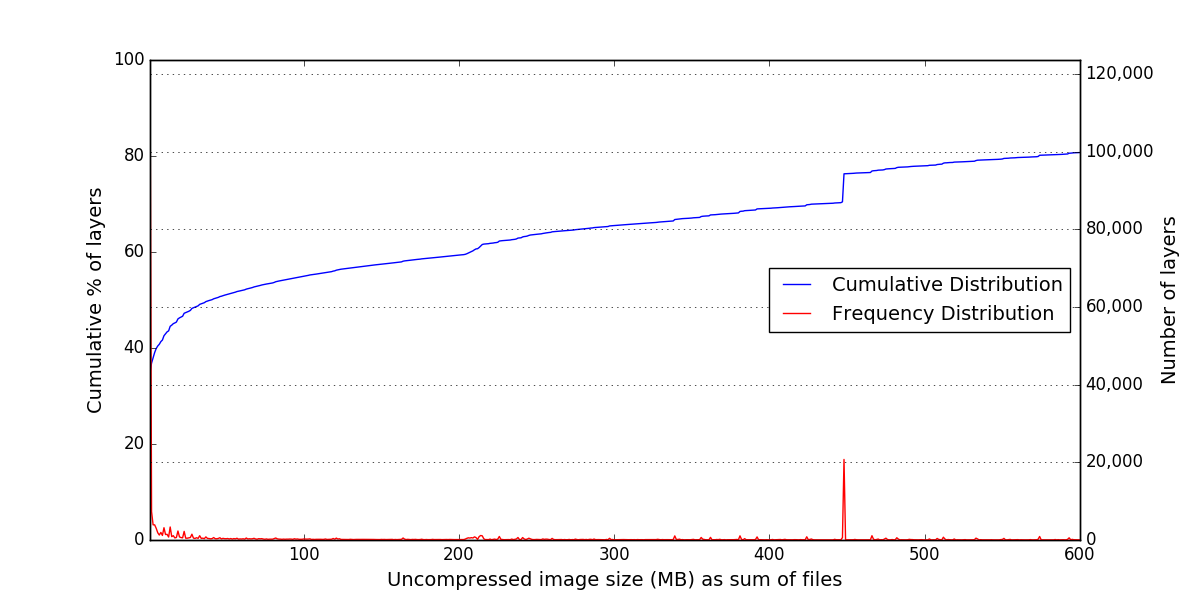
\includegraphics[width=0.5\textwidth]{graphs/distributionUncompressed_image_size_(MB)_as_sum_of_files}\\
	\caption{image decompression size as sum of files}\label{fig_image_size_compression}
\end{figure}

\begin{figure}
	\centering
	% Requires \usepackage{graphicx}
	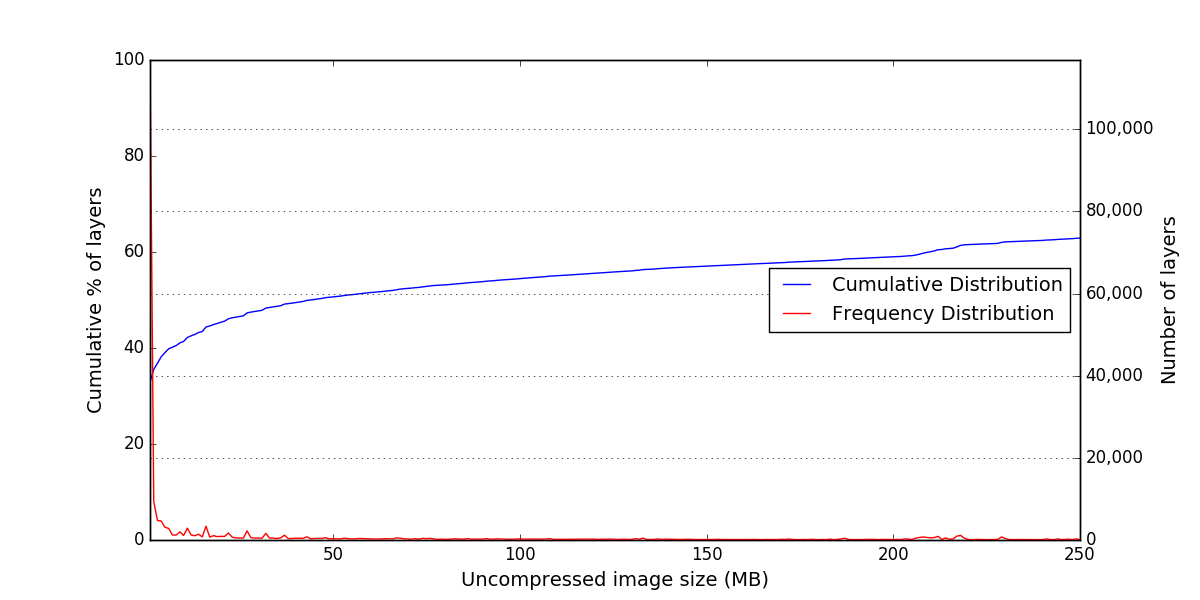
\includegraphics[width=0.5\textwidth]{graphs/distributionUncompressed_image_size_(MB)}\\
	\caption{Image decompression size (archival)}\label{fig_image_size_compression}
\end{figure}

Figure~\ref{fig_image_size_decompression}

\subsubsection{Compression rate distribution}

1. Fig: Compression ratio as the sum of its layer decompression size divided by the sum of its gzip compressed layer size.

\begin{figure}
	\centering
	% Requires \usepackage{graphicx}
	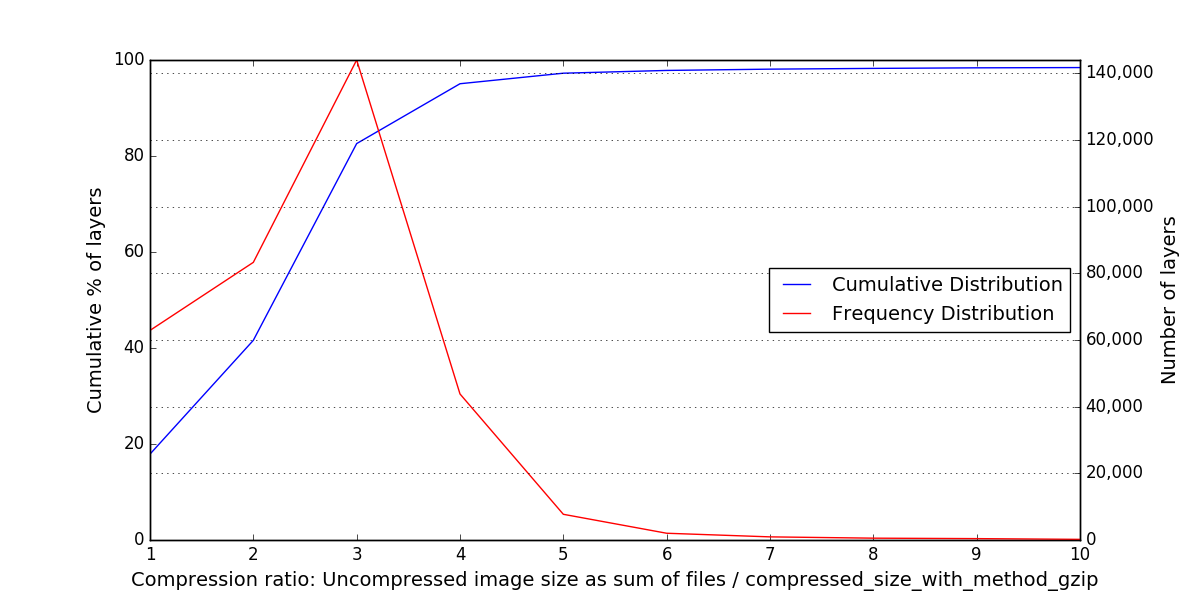
\includegraphics[width=0.5\textwidth]{graphs/distributionCompression_ratio_Uncompressed_image_size_as_sum_of_files_divided_by_compressed_size_with_method_gzip}\\
	\caption{Compression rate}\label{fig_image_size_compression}
\end{figure}

\begin{figure}
	\centering
	% Requires \usepackage{graphicx}
	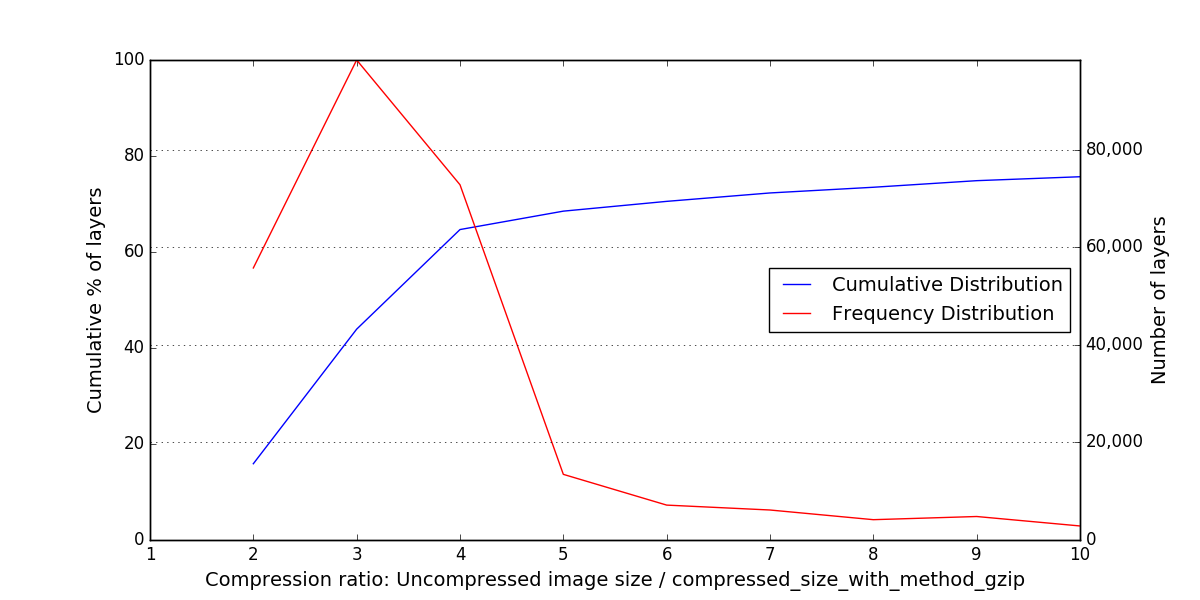
\includegraphics[width=0.5\textwidth]{graphs/distributionCompression_ratio_Uncompressed_image_size_divided_by_compressed_size_with_method_gzip.png}\\
	\caption{Compression rate}\label{fig_image_size_compression}
\end{figure}

\subsubsection{Layer count distribution}

1. Fig: Layer count distribution.


\subsubsection{Repeat layer count distribution}

1. Fig: Repeat layer count distribution.

\begin{figure}
	\centering
	% Requires \usepackage{graphicx}
	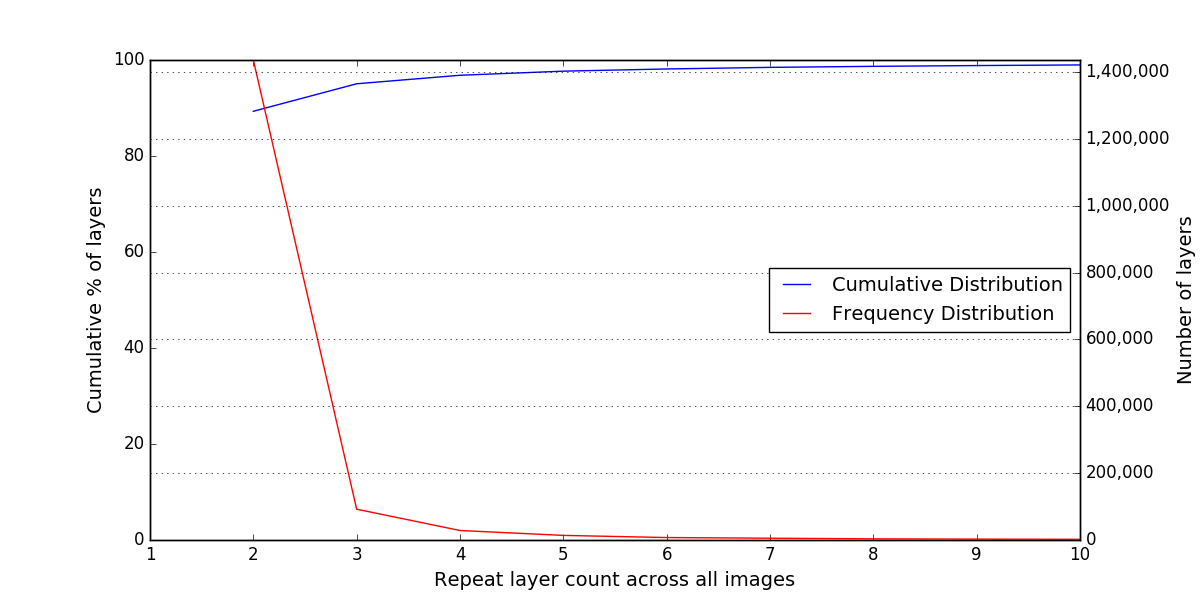
\includegraphics[width=0.5\textwidth]{graphs/distributionRepeat_layer_count_across_all_images}\\
	\caption{Repeat layer count distribution}\label{fig_image_size_compression}
\end{figure}

\subsubsection{File count distribution}

1. Fig: File count distribution.

\begin{figure}
	\centering
	% Requires \usepackage{graphicx}
	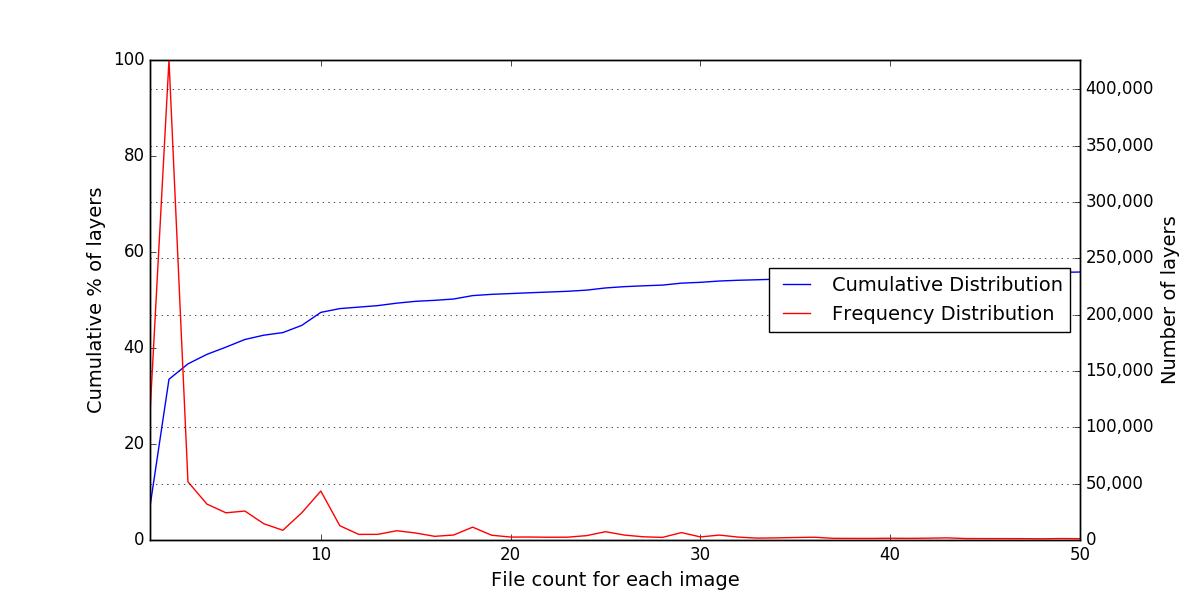
\includegraphics[width=0.5\textwidth]{graphs/distributionFile_count_for_each_image.png}\\
	\caption{File count distribution}\label{fig_image_size_compression}
\end{figure}

\subsubsection{Other metrics, exectution envirnoment}

\subsection{Layer}

\subsubsection{Layer size distribution}

1. Fig: Layer compression size

\begin{figure}
	\centering
	% Requires \usepackage{graphicx}
	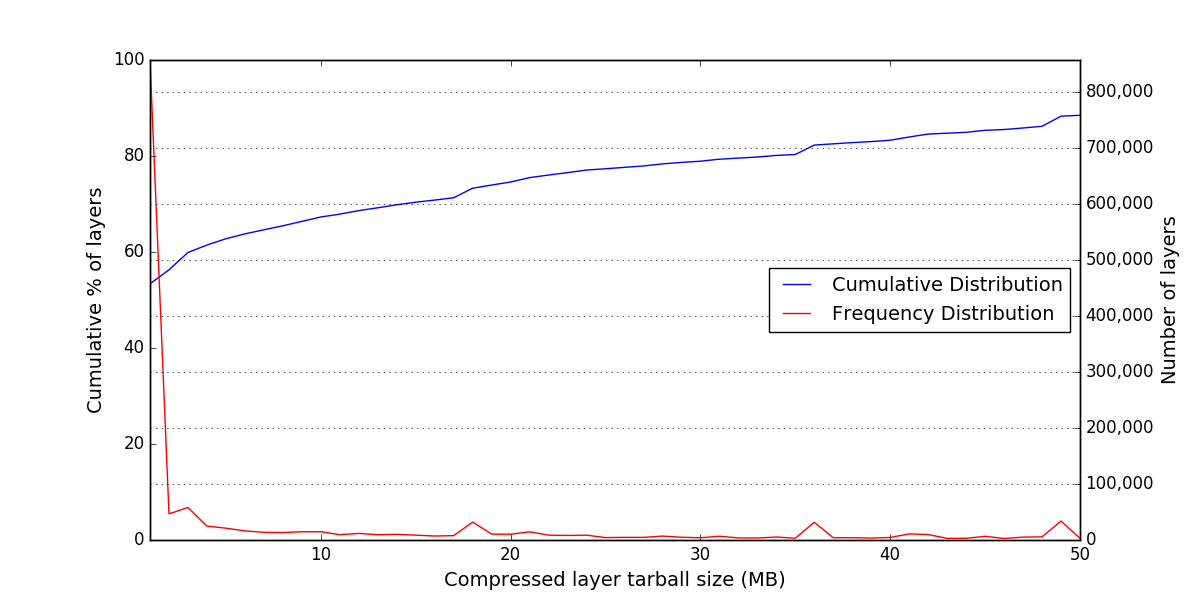
\includegraphics[width=0.5\textwidth]{graphs/distributionCompressed_layer_tarball_size_(MB).png}\\
	\caption{Layer compression size}\label{fig_image_size_compression}
\end{figure}

2. Fig: Layer Decompressed size

\begin{figure}
	\centering
	% Requires \usepackage{graphicx}
	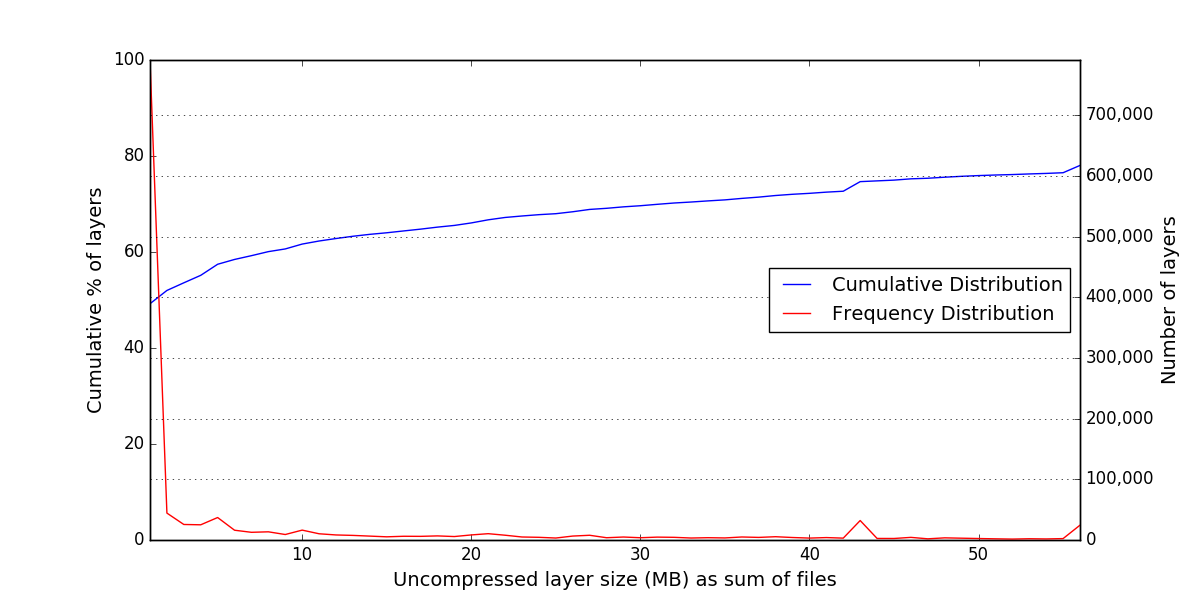
\includegraphics[width=0.5\textwidth]{graphs/distributionUncompressed_layer_size_(MB)_as_sum_of_files.png}\\
	\caption{Layer decompression size (sum of file)}\label{fig_image_size_compression}
\end{figure}

\begin{figure}
	\centering
	% Requires \usepackage{graphicx}
	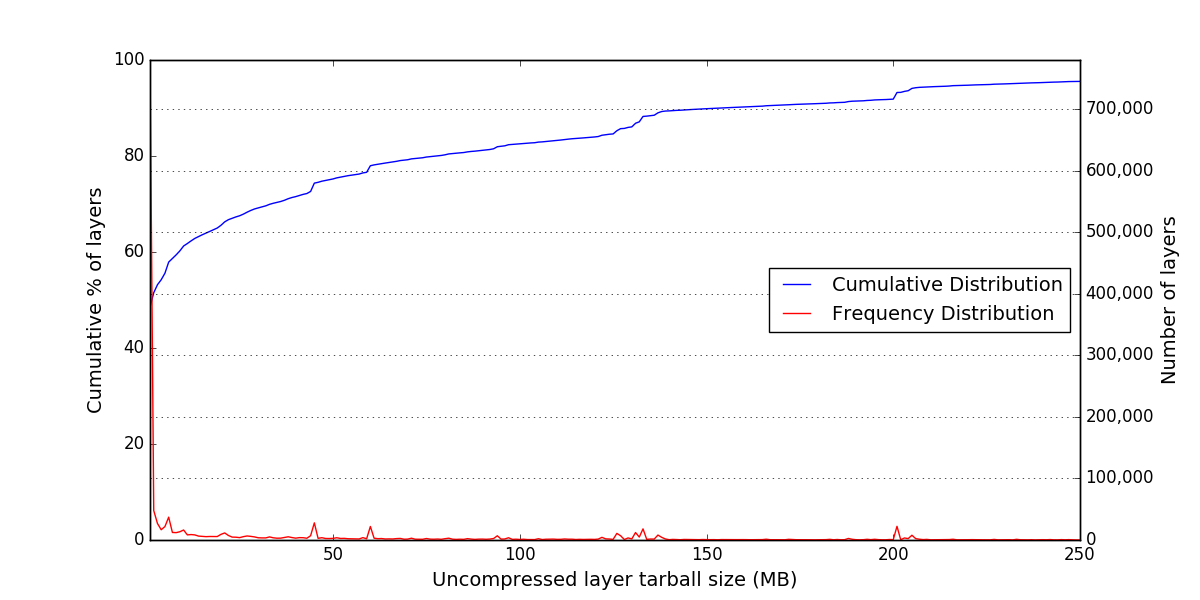
\includegraphics[width=0.5\textwidth]{graphs/distributionUncompressed_layer_tarball_size_(MB).png}\\
	\caption{Layer decompression size (archival)}\label{fig_image_size_compression}
\end{figure}

\subsubsection{Compression rate distribution}

1. Fig: Compression ration as the layer decompression size divided by the gzip compressed layer size.

\begin{figure}
	\centering
	% Requires \usepackage{graphicx}
	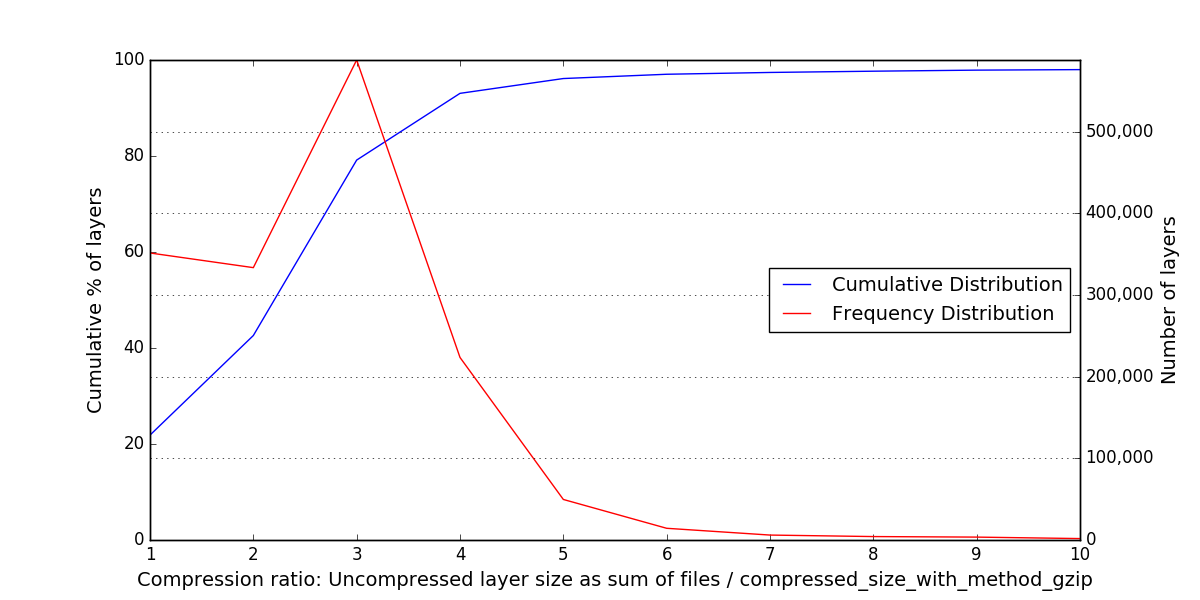
\includegraphics[width=0.5\textwidth]{graphs/distributionCompression_ratio_Uncompressed_layer_size_as_sum_of_files_divided_by_compressed_size_with_method_gzip.png}\\
	\caption{Compression rate}\label{fig_image_size_compression}
\end{figure}

\begin{figure}
	\centering
	% Requires \usepackage{graphicx}
	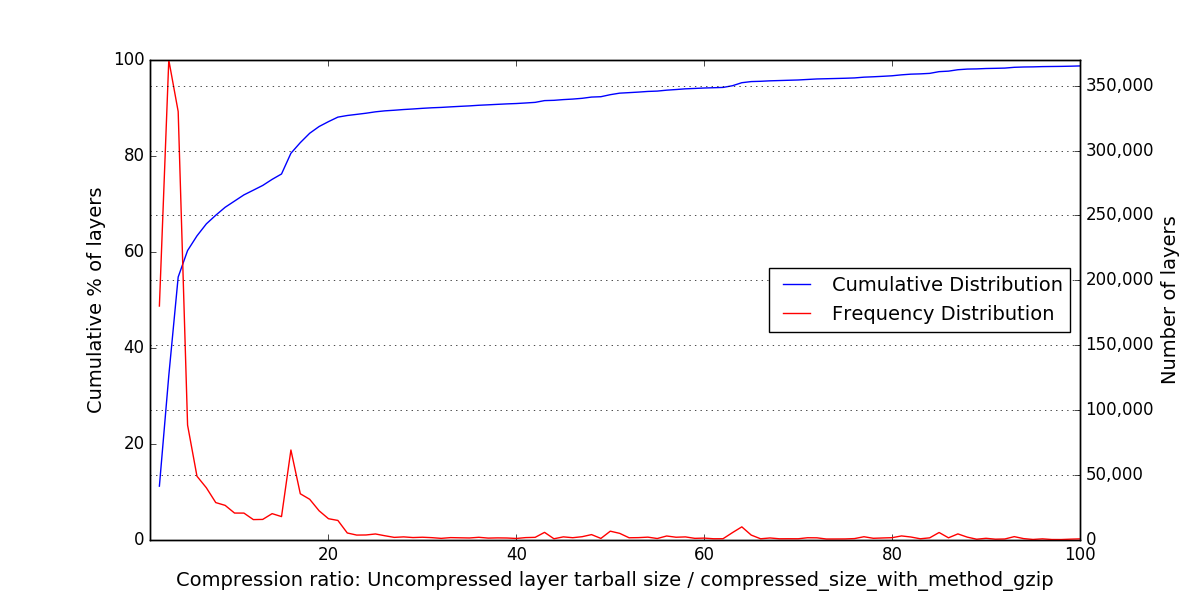
\includegraphics[width=0.5\textwidth]{graphs/distributionCompression_ratio_Uncompressed_layer_tarball_size_divided_by_compressed_size_with_method_gzip.png}\\
	\caption{Compression rate}\label{fig_image_size_compression}
\end{figure}

\subsubsection{Layer depth distribution}

1. Fig: Layer depth

\begin{figure}
	\centering
	% Requires \usepackage{graphicx}
	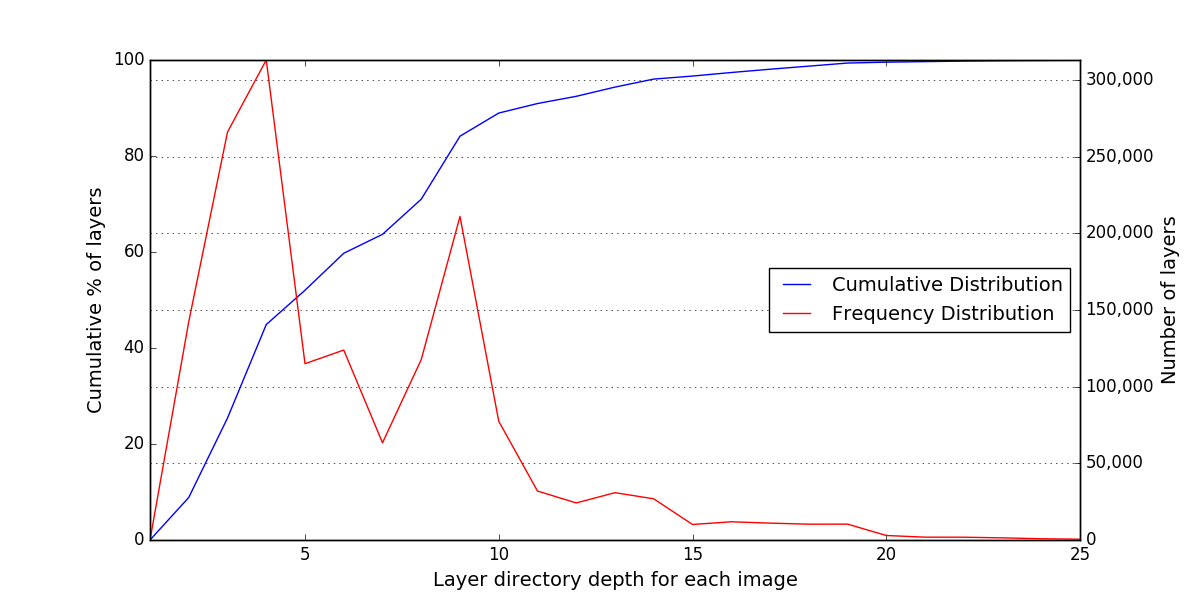
\includegraphics[width=0.5\textwidth]{graphs/distributionLayer_directory_depth_for_each_image.png}\\
	\caption{Layer depth distribution}\label{fig_image_size_compression}
\end{figure}


\subsubsection{File count distribution}

1. Fig: File count distribution.

\subsubsection{Directory count distribution}

1. Fig: Directory count distribution.

\begin{figure}
	\centering
	% Requires \usepackage{graphicx}
	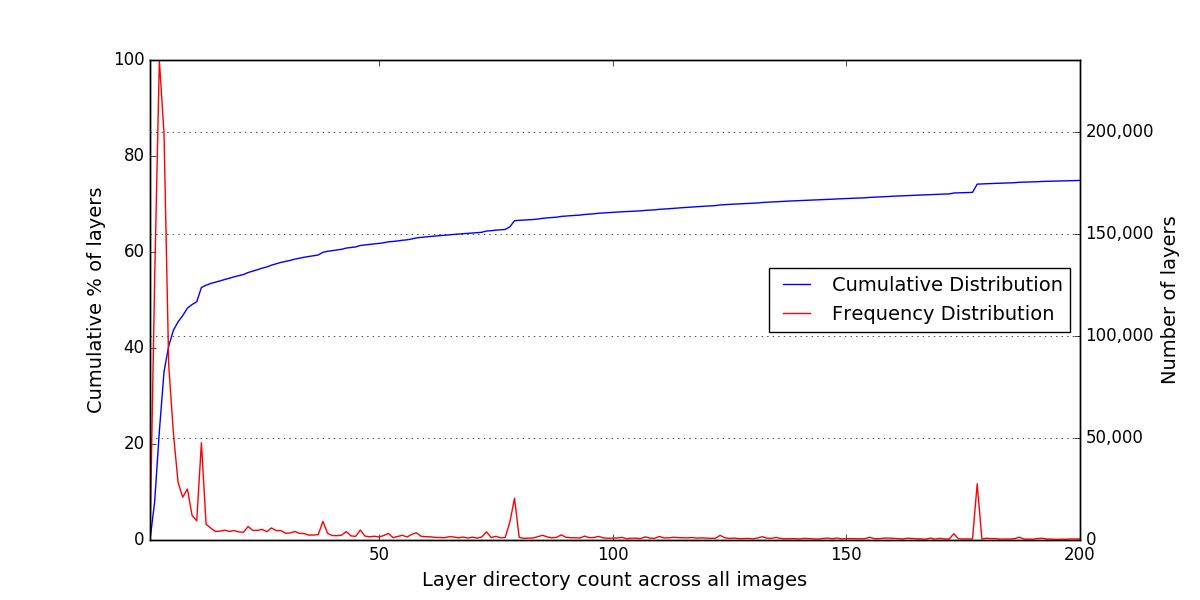
\includegraphics[width=0.5\textwidth]{graphs/distributionLayer_directory_count_across_all_images.png}\\
	\caption{Directory count distribution}\label{fig_image_size_compression}
\end{figure}

\subsubsection{Layer directory depth distribution}

1. Fig: Layer directory depth distribution.


\subsubsection{Other metrics, layer age}

\subsection{File}

%\subsubsection{File count distribution}

\subsubsection{File size distribution}

\subsubsection{File type distribution}

REGTYPE:3006619271
SYMTYPE: 282379663

\begin{figure*}
	\centering
	% Requires \usepackage{graphicx}
	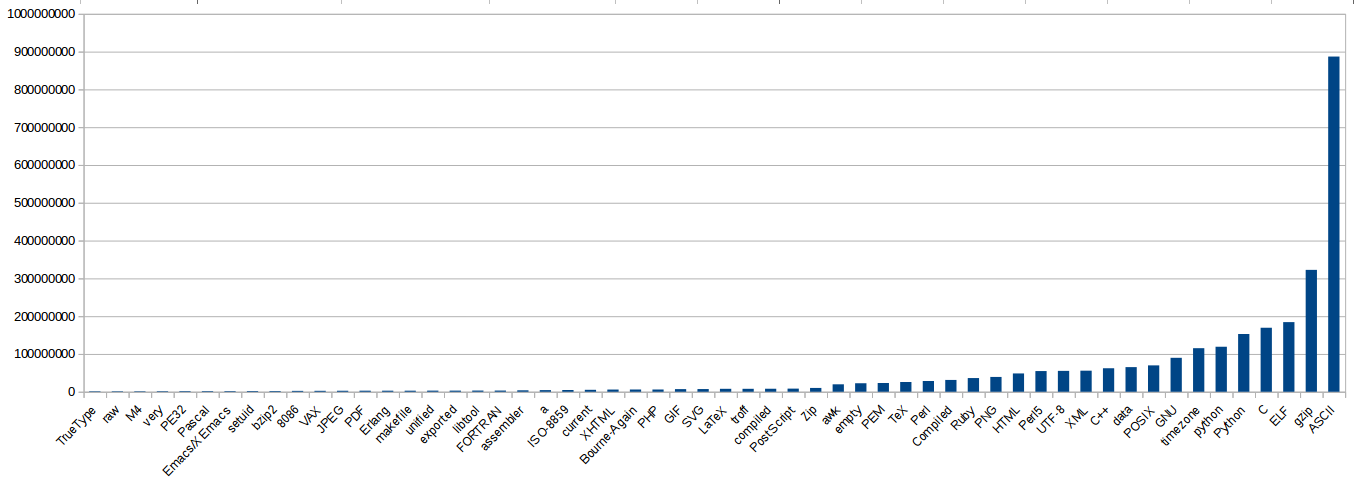
\includegraphics[width=1\textwidth]{graphs/file_type.png}\\
	\caption{file type distribution (archival)}\label{xxx}
\end{figure*}

\subsubsection{Repeat file count distribution}
